\chapter{Results} \label{results}
This chapter will first describe the monitoring and evaluation of the training process. Then a summary of the exhaustive search, followed by the subsets responsible for the highest mean performance per subset size. Finally, all individuals subsets' performance are visualized to better find the most unique subsets. 

\section{Experiment: Exhaustive Search}
    
    \subsection{Training}
        In figure \ref{training_overveiw_fig} an example plot illustrates how the training process was monitored. This example is visually small, but the most important features will now be described. The example comes from the final logging of the model trained on all frequencies.
        \clearpage
        \begin{figure}[H]
             %scale=0.4,

            \hspace*{-3.2cm}
            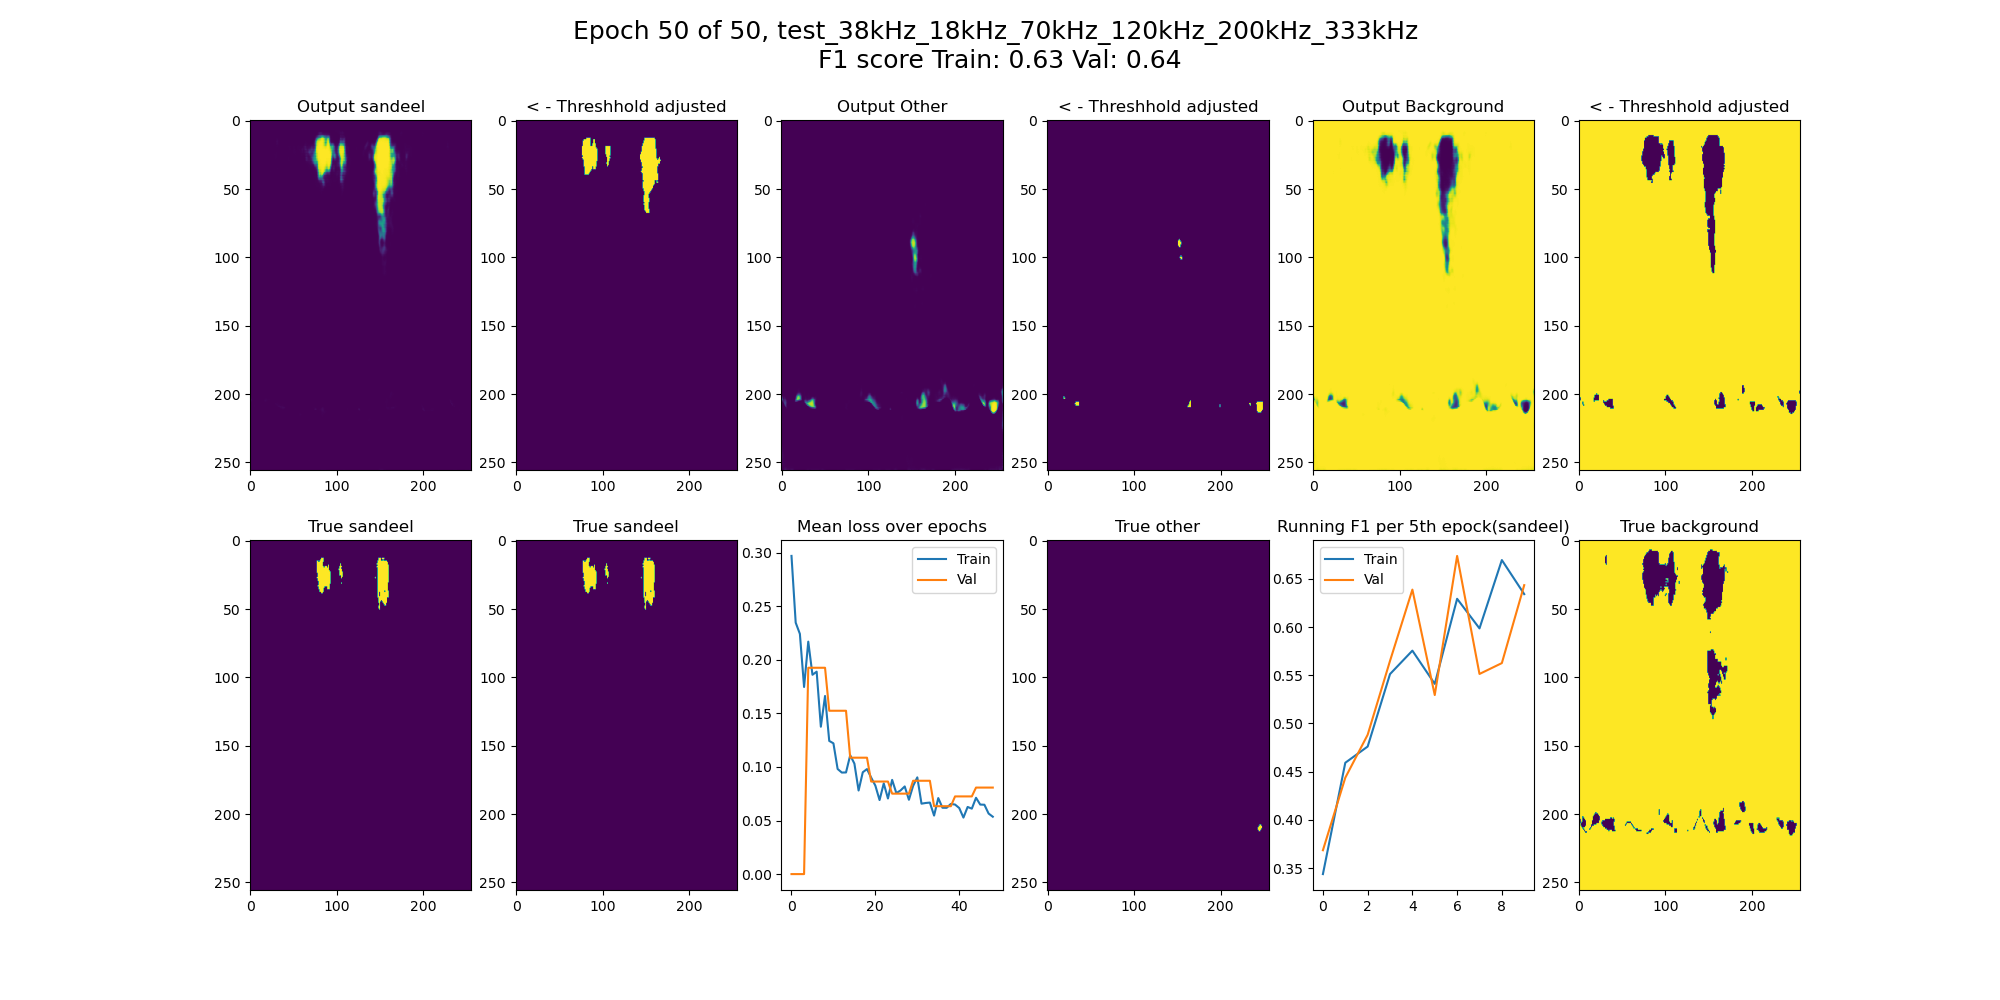
\includegraphics[scale=0.45]{figures/epoch_50_test_38kHz_18kHz_70kHz_120kHz_200kHz_333kHz.png}
            \caption[Training example monitoring]{Example training monitoring. The upper row shows the network's output for each class on a validation sample, with and without a threshold applied. In the lower row, the true values for each class, with the historical loss and F1-score are visualized. Yellow is values close to 1 and purple is 0.}
          	\medskip 
            \label{training_overveiw_fig}
        \end{figure}
        
        
        Extracted from figure \ref{training_overveiw_fig}, figure \ref{loss_f1_duo_plot_fig} shows that both the validation and training loss follow the same trend. The F1-score for validation and training data follows approximately the same values, showing no issues regarding over-/under-fitting. Finally, the visual inspection suggest satisfactory performance of the classifier on the \textit{sandeel} class, as illustrated in figure \ref{sandeel_threshold_label}.%(add more examples to appendix?) 
        
        \clearpage
        \begin{figure}[H]
            \centering
            \subfloat[\centering Loss visualized along the y-axis and the x-axis represent epochs.]{{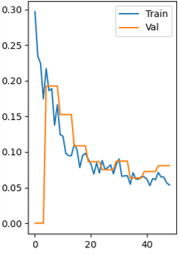
\includegraphics[width=5cm]{figures/Loss_val_train.png} }}%
            \qquad
            \subfloat[\centering F1-score visualized along the y-axis and the x-axis represent epochs.]{{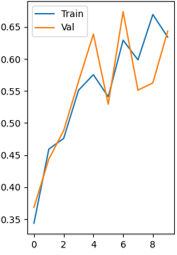
\includegraphics[width=5cm]{figures/F1_score_per_5.png} }}%
            \caption[Loss and F1 score during training]{The F1-score and loss for both training and validation. The validation loss was calculated less often, resulting in larger jumps in value. The training and validation F1-score on the final validation data was respectively 0.63 and 0.64.}%
            \label{loss_f1_duo_plot_fig}%
        \end{figure}
            
        \begin{figure}[H]
            \centering
            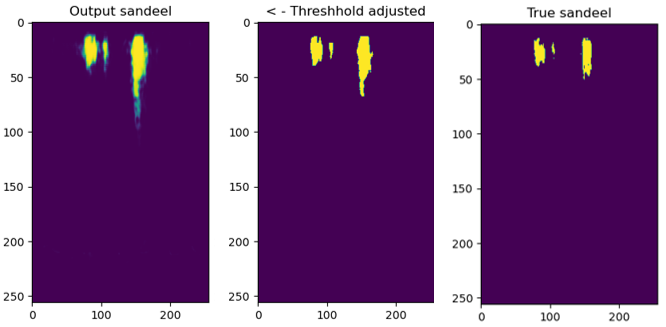
\includegraphics[scale=0.7]{figures/SANDEEL_WITH_LABEL.png}
            \caption[Example output, threshold and label]{From left to right; Network output for the \textit{sandeel} class, same output threshold adjusted, and finally the label for the current sample.}
          	\medskip 
            \label{sandeel_threshold_label}
        \end{figure}
    
    
     By viewing the complete logs from training, some combinations with one or two frequencies likely needed more training to converge. More examples can be found in the appendixes \ref{examples training}.
    

\subsection{Results: Exhaustive Search}
    This section starts with a summary of the subsets' mean F1-score from the 10 tests. Summarized per subset size for minimum F1-score, maximum F1-score and median F1-score in table \ref{summary_per_subset_size_table}. The mean F1-score of all individual subsets can be viewed in appendix \ref{result_all_subsets_table}. Then the frequencies contributing to the highest performing subsets are visualized for F1-score (figure \ref{increasing_freq_f1_score_fig}), precision (figure \ref{increasing_freq_precision_score_fig}) and recall (figure \ref{increasing_freq_recall_score_fig}).


    % Please add the following required packages to your document preamble:
% \usepackage{longtable}
% Note: It may be necessary to compile the document several times to get a multi-page table to line up properly
\begin{longtable}{llllllll}
\caption{This table shows a summary of the mean performance for each size of subsets over the ten tests. Min and median increases with the subset size, but the max performance stagnates after a subset size of three is reached. }\\
                  &      &      &      &      &      &      &  \\ \hline
\endfirsthead
%
\endhead
%
\hline
\endfoot
%
\endlastfoot
%
\textbf{Subset size:}      & \textbf{1}    & \textbf{2}    & \textbf{3}    & \textbf{4}    & \textbf{5}    & \textbf{6}    &  \\ \hline
F1-score (min):   & 0.25 & 0.28 & 0.34 & 0.42 & 0.50 & 0.66 &  \\
%F1-score (mean)   & 0.29 & 0.38 & 0.46 & 0.53 & 0.61 & 0.66 &  \\
F1-score (median) & 0.28 & 0.37 & 0.45 & 0.54 & 0.62 & 0.66 &  \\
F1-score (max):   & 0.34 & 0.46 & 0.65 & 0.67 & 0.67 & 0.66 &  \\ \hline
\label{summary_per_subset_size_table}

\end{longtable}
    
        
        \begin{figure}[H]
            \centering
            %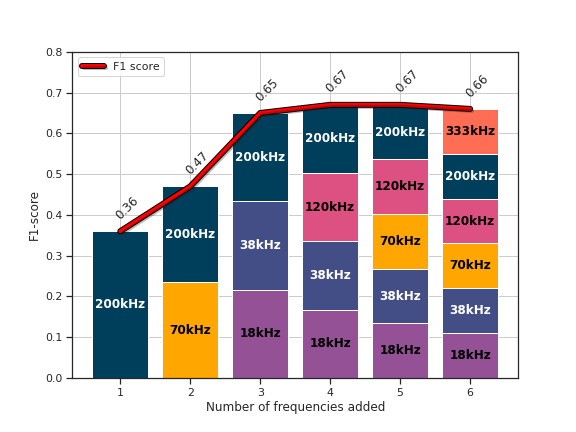
\includegraphics[scale=0.7]{figures/increasing_freq_f1.png}
            \includesvg[inkscapelatex=false,width=0.9\textwidth,keepaspectratio]{figures/increasing_freq_f1.svg}
            \caption[Best frequency combination - F1-score]{The highest performing frequency subset based on mean F1-score is visualized. The most drastic increase in performance happens with the three frequencies \textit{18kHz}, \textit{38kHz} and \textit{200kHz}.}
          	\medskip 
            \label{increasing_freq_f1_score_fig}
        \end{figure}

        \clearpage
        % Precision
        \begin{figure}[H]
            \centering
            %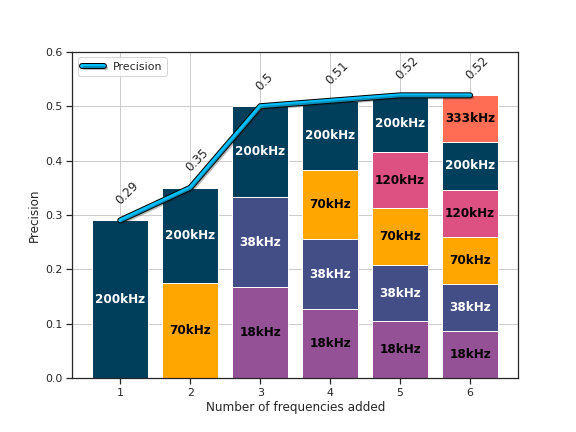
\includegraphics[scale=0.7]{figures/increasing_freq_precision.png}
            \includesvg[inkscapelatex=false,width=0.9\textwidth,keepaspectratio]{figures/increasing_freq_precision.svg}
            \caption[Best frequency combination - Precision]{The best performing frequency subset based on mean precision is visualized. The trend is similar to the one based on F1-score.}
          	\medskip 
            \label{increasing_freq_precision_score_fig}
        \end{figure}
        
        \clearpage
        %\clearpage
        \begin{figure}[H]
            \centering
            %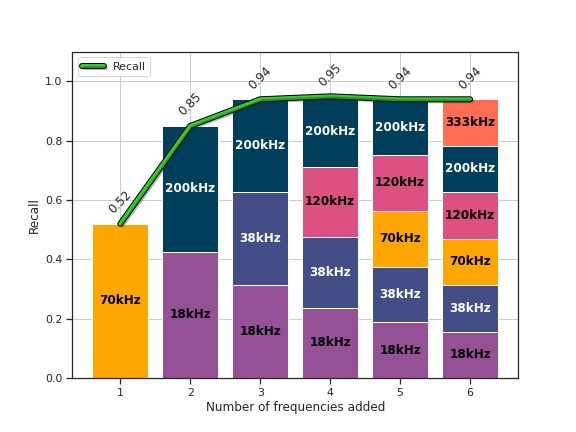
\includegraphics[scale=0.7]{figures/increasing_freq_recall.png}
            \includesvg[inkscapelatex=false,width=0.9\textwidth,keepaspectratio]{figures/increasing_freq_recall.svg}
            \caption[Best frequency combination - Recall]{The best performing frequency subset based on mean recall is visualized. The steep increase in performance happens already at two frequencies. Indicating that the best combination at this stage already finds most of the \textit{sandeel} class.}
          	\medskip 
            \label{increasing_freq_recall_score_fig}
        \end{figure}

    \subsection{Individual Subsets}
        Figure \ref{errorbar_fig} illustrates a complete plot of all error bars, with sections for each test. The plot has no complete overview over which frequencies belong to which result, only a red circle encompassing the error bar related to the subset \textit{18},\textit{38} and \textit{200kHz}. This combination outclasses all other subset in the same and previous tests, and competes with all the results later achieved. In all other sections, no subset stands out in regard to F1-score.
        \begin{figure}[H]
            \centering
            %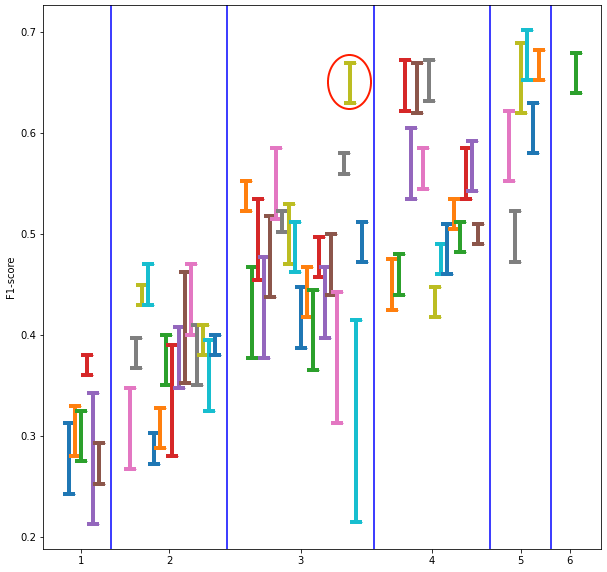
\includegraphics[scale=0.7]{figures/error_bar.png}
            \includesvg[inkscapelatex=false,width=1\textwidth,keepaspectratio]{figures/all_combinations.svg}
            \caption[Error bars per combination]{Each colored error bar represents a frequency-subset. The error bar's highest y-value is the max value achieved for this subset from all 10 tests, and the bottom the lowest. Blue vertical lines group the error bars by the subsets size, and the black dots are the mean performance of the subset.}
          	\medskip 
            \label{errorbar_fig}
        \end{figure}
    
        To further analyze the performance of the unique subset \textit{18kHz}, \textit{38kHz}, and \textit{200kHz}, two new subsets were created. The first with subsets which at a minimum contained the aforementioned frequencies. In the second, these eight subsets were removed, and then the eight best performing from this set were extracted. These subsets are visualized in figure \ref{with_without_figure}.
        
        \begin{figure}[H]
            \centering
            %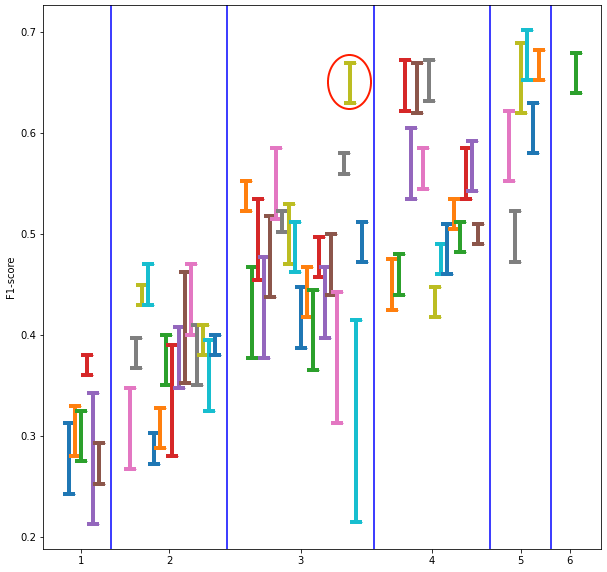
\includegraphics[scale=0.7]{figures/error_bar.png}
            \includesvg[inkscapelatex=false,width=0.7\textwidth,keepaspectratio]{figures/with_without.svg}
            \caption[With and without unique subset]{In this figure, the mean F1-score of all subsets containing 18kHz, 38kHz, and 200kHz is plotted as a blue line (Eight in total). The orange line is the eight highest performing subsets from a set where the subset 18kHz, 38kHz, and 200kHz is not included in any subset. The figure show that all the highest performing subsets include the frequencies \textit{18kHz}, \textit{38kHz}, and \textit{200kHz}.}
          	\medskip 
            \label{with_without_figure}
        \end{figure}
        
        
    \subsection{Performance Trend per Frequency}
        In this section, the performance trend for each frequency is visualized. For each frequency, all subsets it was part of were extracted, and then sorted in increasing order of mean F1-score. Visualized in figure \ref{performance_trend_fig}.
        
        \begin{figure}[H]
            \centering
            %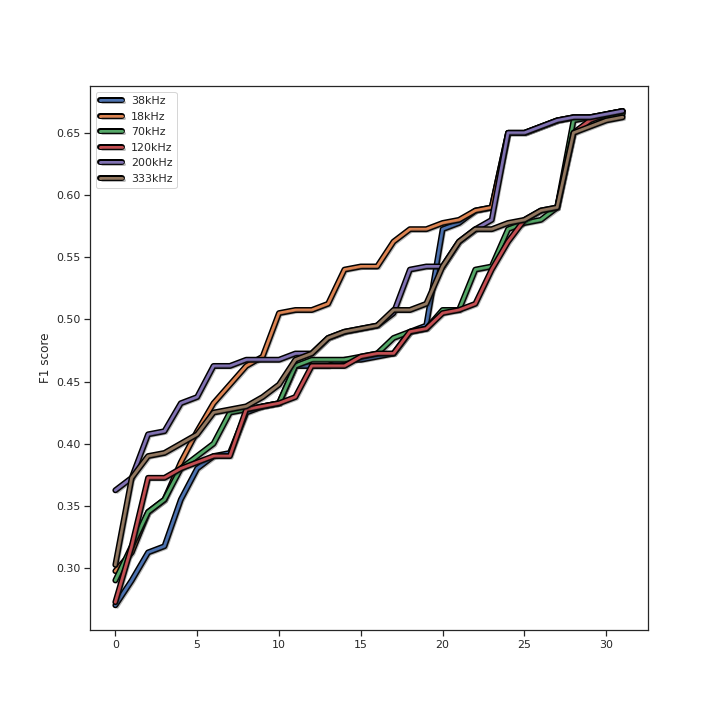
\includegraphics[scale=0.7]{figures/perfomance_trend.png}
            \includesvg[inkscapelatex=false,width=0.9\textwidth,keepaspectratio]{figures/perfomance_trend.svg}
            \caption[Performance trend per frequency]{This figure illustrates the performance trend of each frequency. From right to left, the plot shows that \textit{18kHz}, \textit{38kHz} and \textit{200kHz} all are part of many combinations with high F1-scores, as seen earlier in figure \ref{increasing_freq_f1_score_fig}. The remaining frequencies quickly fall in performance, most likely due to not being paired with any of the three previously mentioned. Looking further to the left, \textit{18kHz} seems to have participated in many combinations on average, resulting in high F1-scores, followed closely by \textit{200kHz}.}
          	\medskip 
            \label{performance_trend_fig}
        \end{figure}
        
        
    

    
    
